\section{What equipment you'll need}
\label{sec:PiEquiptment}

	The Raspberry Pi is a full personal computer on a single board, so we can think of it as a replacement for an old tower-style desktop machine.
	
	To get the Raspberry Pi working then, we need to add the same peripherals as we would with a desktop machine:
	
	\begin{itemize}[nosep]
		\item A TV/computer \textbf{monitor}, to output to.
		\item A \textbf{keyboard} and \textbf{mouse} for input.
	\end{itemize}
		
	In addition, the Raspberry Pi also requires:
	\begin{itemize}[nosep]
		\item A \textbf{Micro USB power supply}, the type used to charge most Smartphones and Tablets.
		\item An 8GB or larger \textbf{MicroSD card}.
	\end{itemize}
	
	\subsection*{Monitor}
	
		The Raspberry Pi uses HDMI for display output. Most modern TVs and monitors will have a HDMI port. You'll need a standard HDMI cable to connect them.
		
		\begin{figure}[h]
			\centering
			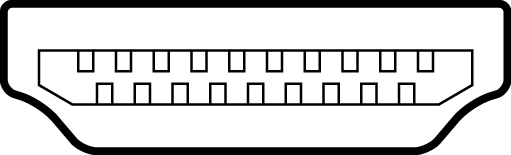
\includegraphics[height=22pt]{McrRaspJam/000_IntroToPi/1_EquipmentNeeded/HDMI}
			\\A HDMI connector
		\end{figure}
		
		If you're using a computer monitor that is a few years old, it may only have a DVI port. In this case, you can use a DVI-HDMI cable to connect to the Raspberry Pi, which can be cheaply purchased.
	
		\begin{figure}[h]
			\centering
			
\includegraphics[height=22pt]{McrRaspJam/000_IntroToPi/1_EquipmentNeeded/DVI}
			\\A typical DVI connector
		\end{figure}
		
		If possible, avoid using VGA connections. They require an (expensive) active adaptor, and are an analogue connector, so produce poorer image quality.
		
		\begin{figure}[h]
			\centering
			
\includegraphics[height=22pt]{McrRaspJam/000_IntroToPi/1_EquipmentNeeded/VGA}
			\\A VGA connector
		\end{figure}

	\subsection*{Keyboard and mouse}
	
		You can use any standard USB keyboard and mouse.
		
		The Linux Operating System that the Raspberry Pi runs also has great compatibility with most wireless peripherals that use a USB dongle, or for Pi 3 the built-in Bluetooth.
		
	\subsection*{Power Supply}
	
		Most phone chargers will boot a Pi, but if you're using add-on boards or multiple USB peripherals, you may run into power issues.
		
		Check the rating on your power supply, \url{raspberrypi.org} recommends an output rating of 5V 1.2A for a Gen1 Pi, and 5V 2.5A for a Pi 3.
		
	\subsection*{MicroSD Card}
	
		The Raspberry Pi does not have a built in ``Hard drive'' like a desktop tower, so the operating system and files are all stored on a MicroSD card.
		
		Your card will need to be \textbf{at least 8GB}, and is recommended to have a speed class of SDHC \textbf{class 10}, denoted by either the ``C10'' logo or a ``U'' logo of any number.
	
		\begin{figure}[h]
			\centering
			
\includegraphics[height=22pt]{McrRaspJam/000_IntroToPi/1_EquipmentNeeded/SDclass10}
			\hspace{12pt}
			
\includegraphics[height=22pt]{McrRaspJam/000_IntroToPi/1_EquipmentNeeded/UHSclass}
			\\SDHC Class 10 \& UHS Class 1
		\end{figure}